\documentclass[zihao=-4, a4paper]{ctexart}

\usepackage[top=2.6cm, bottom=2.4cm, left=2.5cm, right=2.5cm]{geometry}
\usepackage{fancyhdr}
\usepackage{booktabs}
\usepackage{array}
\usepackage{tabularx}
\usepackage{graphicx}
\usepackage{float}
\usepackage{enumitem}
\usepackage[labelfont=bf, font=small, skip=4pt]{caption}
\usepackage{xcolor}
\usepackage[hidelinks, bookmarks=true, bookmarksnumbered=true]{hyperref}

\setCJKmainfont{Songti SC}
\setCJKsansfont{Heiti SC}
\setCJKfamilyfont{hei}{Heiti SC}
\newcommand{\hei}{\CJKfamily{hei}}
% 圆圈数字①②③等交给中文字体渲染(拉丁字体无此字形)
\xeCJKDeclareCharClass{CJK}{"2460 -> "24FF}

\linespread{1.45}
\setlength{\parindent}{2em}
\setlength{\parskip}{2pt}

\ctexset{
  section = {format = \raggedright\hei\zihao{4}, aftername = \quad, beforeskip = 14pt, afterskip = 8pt},
  subsection = {format = \raggedright\hei\zihao{-4}, aftername = \quad, beforeskip = 10pt, afterskip = 5pt},
}

\pagestyle{fancy}
\fancyhf{}
\fancyhead[C]{\small\color{gray} 知心陪练 PeerCoach · 过程性证明材料}
\fancyfoot[C]{\small\thepage}
\renewcommand{\headrulewidth}{0.4pt}
\renewcommand{\footrulewidth}{0pt}

% 待补拍照片占位框(虚线)
\usepackage{tikz}
\newcommand{\photobox}[1]{%
  \par\vspace{6pt}\noindent
  \begin{tikzpicture}
  \node[draw=gray!55, dashed, line width=0.8pt, rounded corners=2pt,
        minimum width=\linewidth, minimum height=2.6cm, inner sep=10pt,
        align=center, text=gray!65, font=\small] {#1};
  \end{tikzpicture}\par\vspace{6pt}}

% 本阶段产出条
\newcommand{\phaseout}[1]{%
  \par\vspace{4pt}\noindent\colorbox{green!8}{\parbox{\dimexpr\linewidth-2\fboxsep}{%
  \small\color{green!35!black}\textbf{本阶段产出:}#1}}\par\vspace{4pt}}

\renewcommand{\arraystretch}{1.3}
\newcolumntype{Y}{>{\raggedright\arraybackslash}X}
\renewcommand{\figurename}{图}
\renewcommand{\tablename}{表}

\begin{document}

% ======================= 封面 =======================
\thispagestyle{empty}
\begin{center}
\vspace*{2cm}
{\zihao{4} 2025—2026 学年全国青少年心理成长知识与应用创新大赛}\\[6pt]
{\zihao{-4} 「小小心理学家」创新大赛 \quad 智能体应用方向}\\[3cm]

{\hei\zihao{0} 知心陪练\ PeerCoach}\\[14pt]
{\hei\zihao{3} ——基于标准化来访者的青少年朋辈心理互助训练智能体}\\[2.4cm]

{\hei\zihao{2} 过程性证明材料}\\[3cm]

{\zihao{4}
\begin{tabular}{rl}
参赛选手: & 陈家治 \\[10pt]
所在学校: & 浙江省杭州第二中学 \\[10pt]
指导教师: & 边玉臣、陈陈 \\
\end{tabular}}\\[2.4cm]

{\zihao{4} 2026 年 7 月}
\end{center}
\clearpage

% ======================= 说明 =======================
\section*{说明}
\addcontentsline{toc}{section}{说明}
本材料按研发时间顺序呈现各阶段的过程证据与说明。文中所有系统界面图均为作品真实运行截图(含接入 DeepSeek 大模型后的真实会谈画面),数据图表均来自真实采集,不摆拍、不虚构。

\subsection*{研发历程总览}
\begin{table}[H]\centering
\caption{研发阶段与产出物一览(具体日期以实际研发记录为准)}
\small
\begin{tabularx}{\textwidth}{@{}p{1.7cm} Y Y >{\centering\arraybackslash}p{2.1cm}@{}}
\toprule
\hei 阶段 & \hei 主要工作 & \hei 产出物 & \hei 时间 \\
\midrule
① 调研分析 & 问卷调研、访谈心理老师、同类作品分析 & 《朋辈互助现状问卷》及统计、需求清单 & 5.26—5.29 \\
② 方案设计 & 理论研读、架构设计、案例剧本与量规编写 & 系统架构图、四案例剧本、五维量规 & 5.30—6.3 \\
③ 系统开发 & 扣子端双智能体搭建、网页训练场编码 & 双智能体应用、网页端(约 1200 行) & 6.4—6.12 \\
④ 调试优化 & 六场景用例测试、试玩反馈迭代 & 调试记录、场景测试通过记录 & 6.13—6.16 \\
⑤ 训练实验 & 前后测实验、问卷回收、数据统计 & 前后测答卷与盲评记录、数据表 & 6.17—6.30 \\
⑥ 验收整理 & 全功能走查、材料整理、成品打包 & 参赛材料包 & 7.1—7.4 \\
\bottomrule
\end{tabularx}
\end{table}

% ======================= 一、步骤 =======================
\section{制作过程步骤}

\subsection{步骤 1:前期调研与需求分析}
围绕「同学倾诉时,你会怎么回应」设计《朋辈互助现状问卷》,面向本校学生与心理委员发放;同时访谈学校心理老师,重点了解心理委员培训的现状与困难。调研确认三个事实:同学间倾诉高频发生;绝大多数学生「愿意帮但不知道怎么回应」;心理委员普遍未接受过系统的回应训练。据此把作品方向从最初构想的「AI 安慰学生」调整为「训练学生成为接得住的人」——这次方向调整是整个作品最关键的一步。共回收有效问卷 200 份(普通同学 160、心理委员 40),结果印证:78.0\% 的学生被同学倾诉过,68.0\% 面对倾诉「不知道怎么回应」,完全没受过训练的高达 82.0\%,而知道危机正确处理步骤的仅 15.0\%——「有岗位、缺训练」得到数据支撑(详见设计报告第 8.1 节)。
\phaseout{《朋辈互助现状问卷》(200 份)、分组统计表、访谈记录、需求清单}

\subsection{步骤 2:方案设计与理论准备}
研读标准化病人方法、艾维助人微技巧、伊根助人模型与守门人训练资料,完成三项设计:一是「案例智能体演、督导智能体评」的双智能体架构与三层系统架构;二是四个分级案例的双层剧本(表层困扰+隐藏层)与《案例编写规范》;三是五维评分量规的三档行为锚点。理论内容同步转写为面向学生的五节「互助微课」。

\begin{figure}[H]\centering
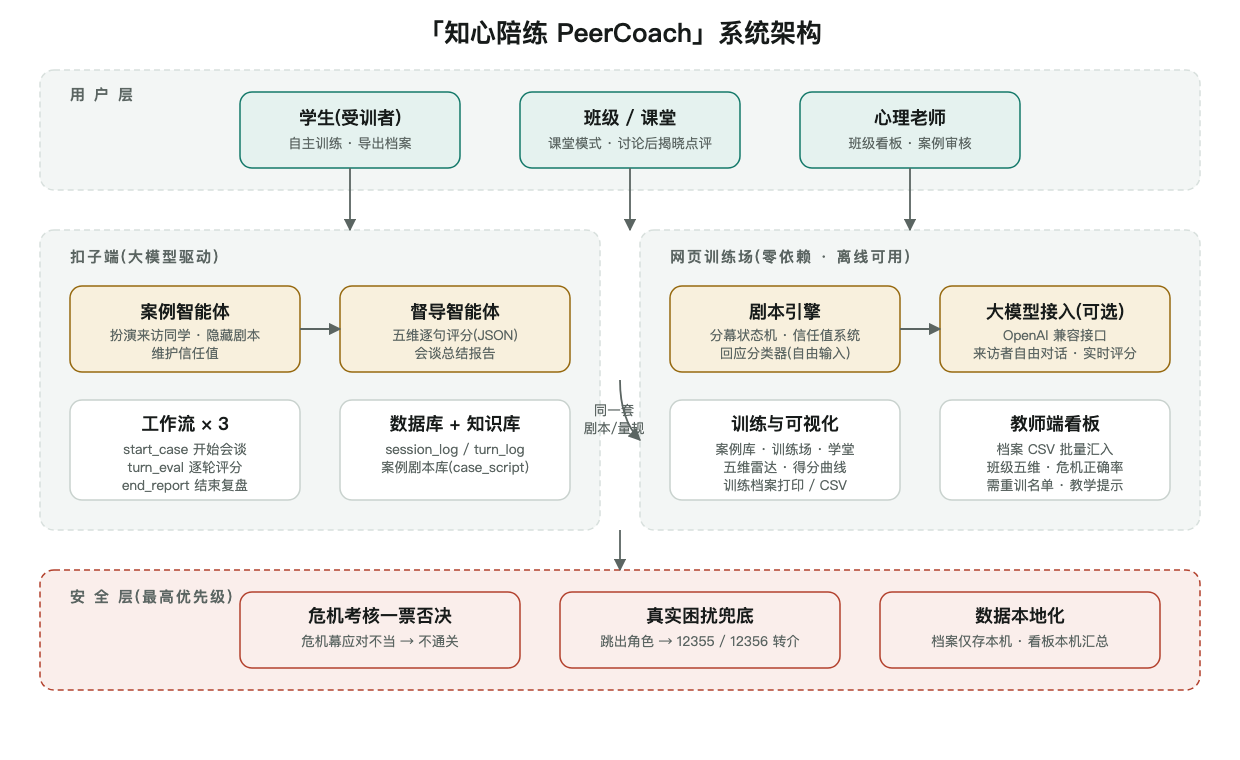
\includegraphics[width=0.9\textwidth]{arch.png}
\caption{系统架构设计图(设计阶段定稿)}
\end{figure}

\begin{figure}[H]\centering
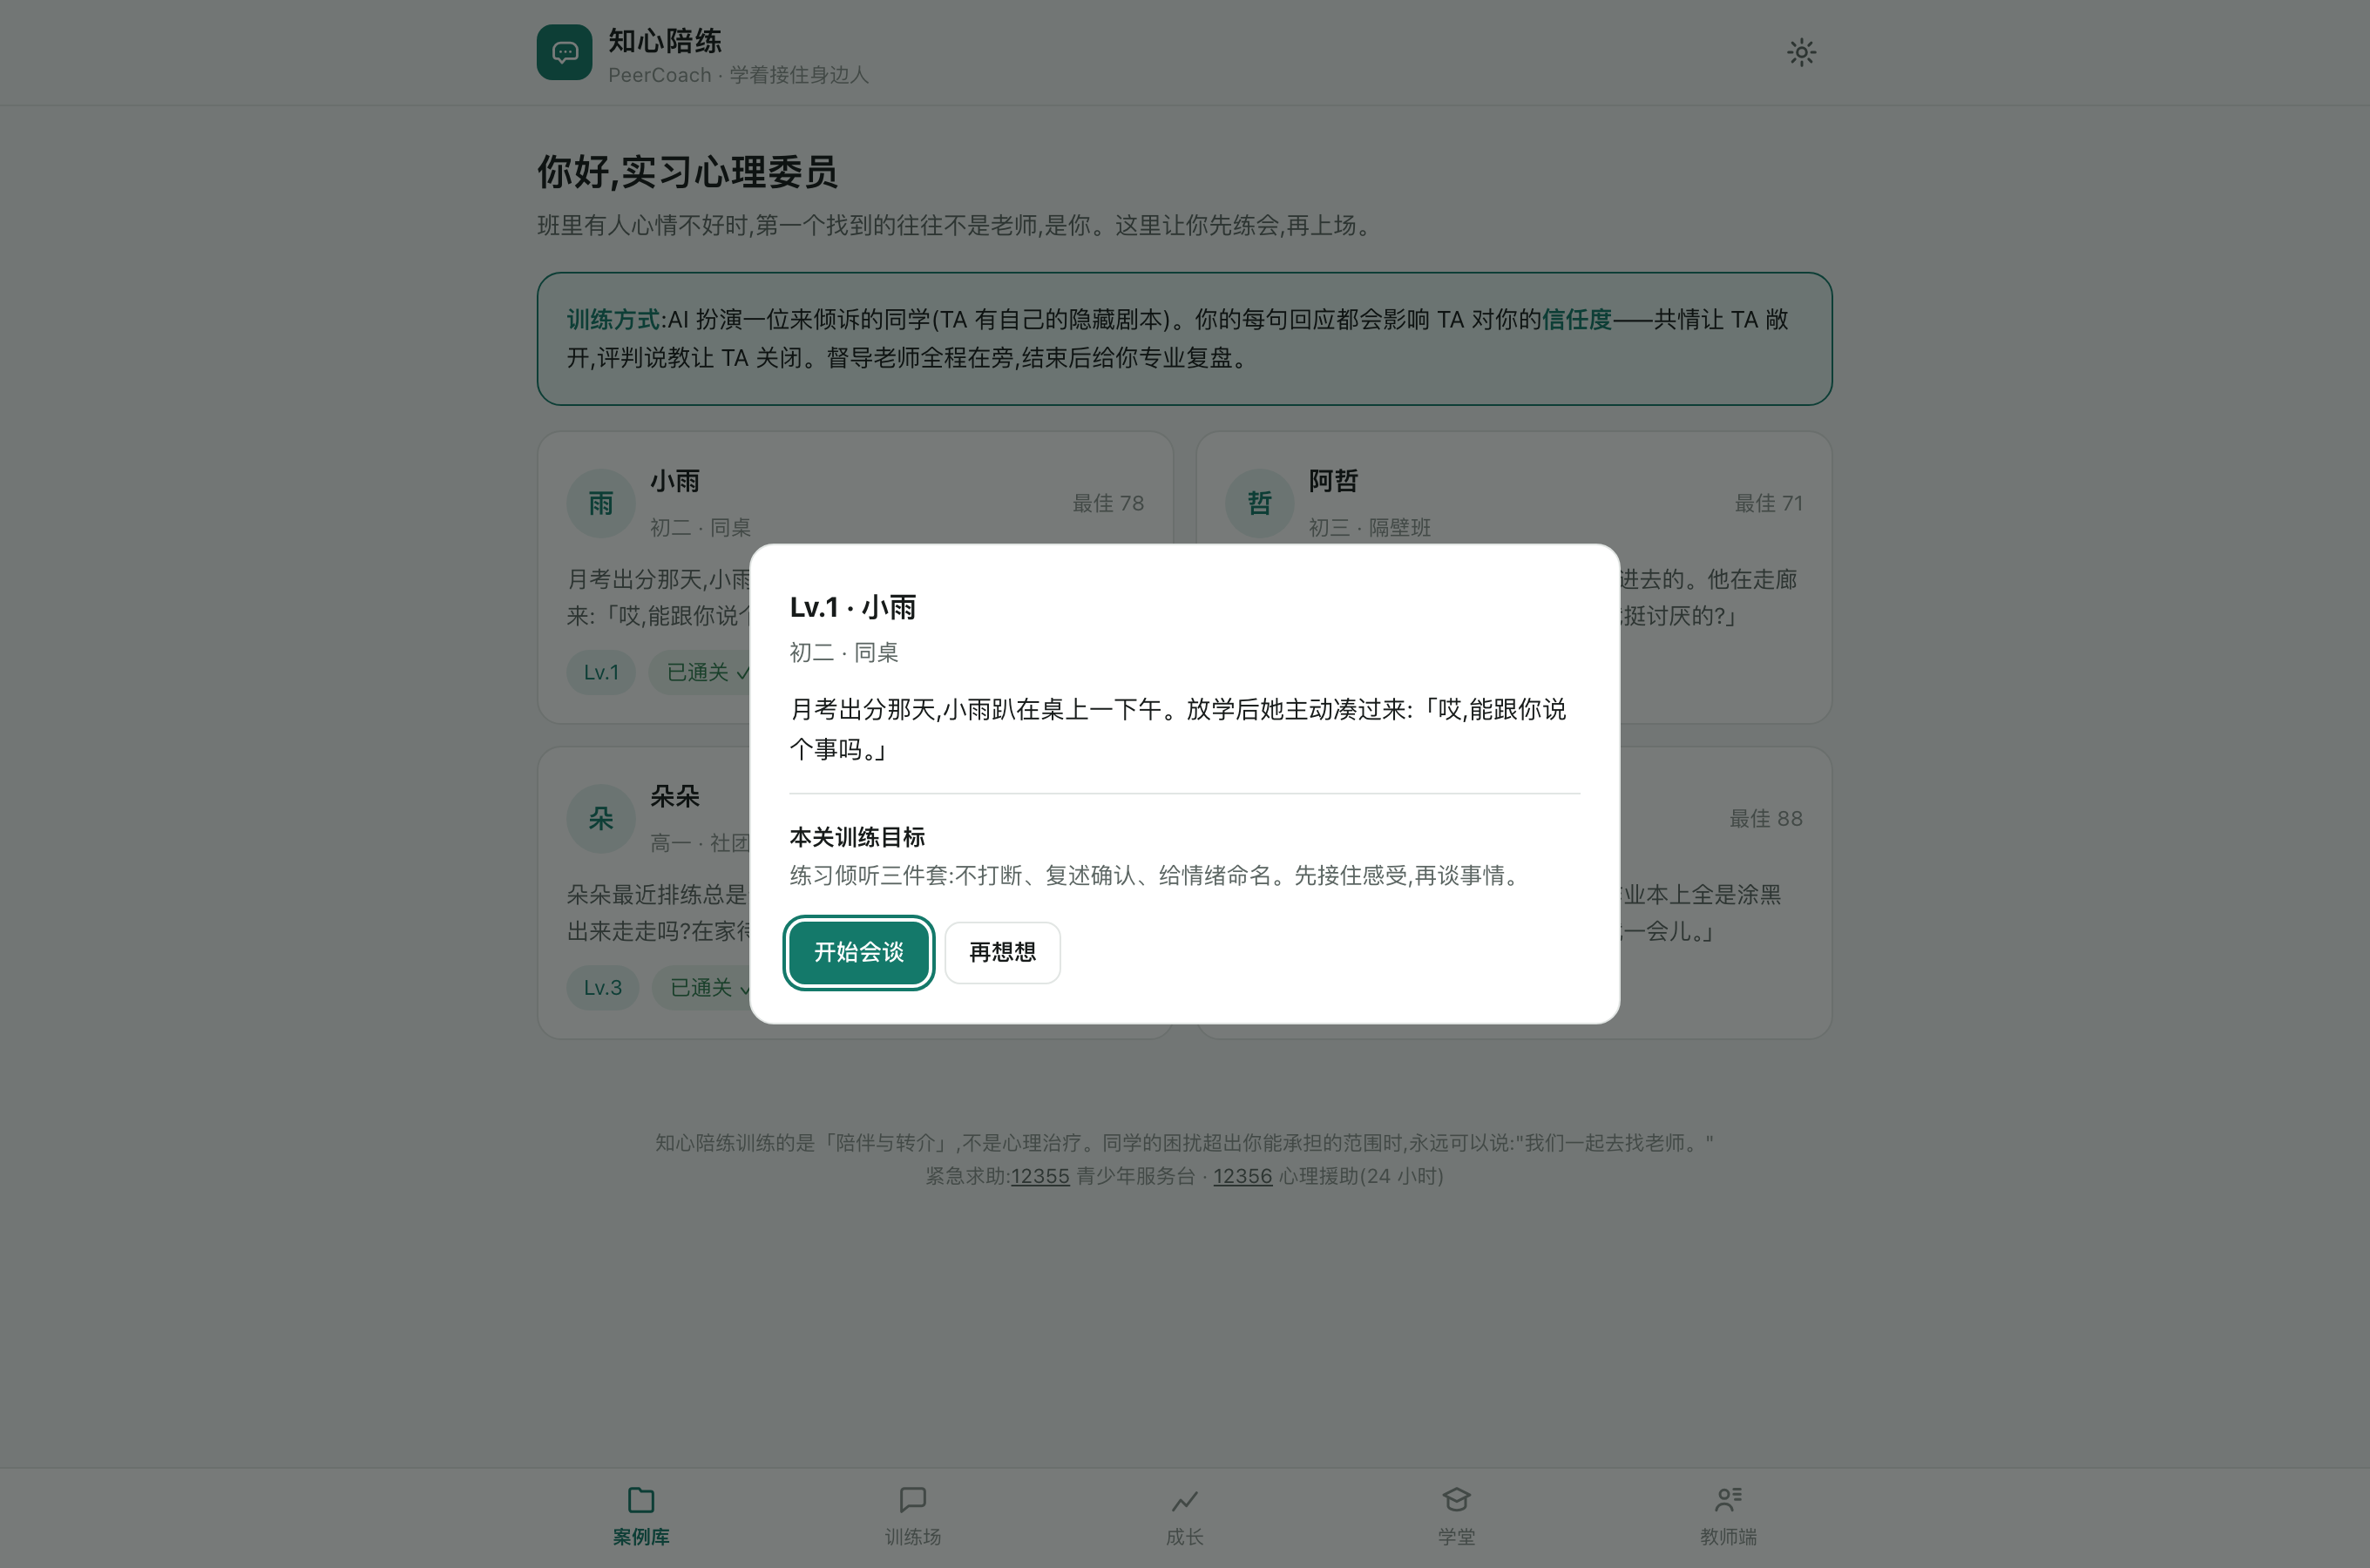
\includegraphics[width=0.86\textwidth]{案例简报.png}
\caption{案例设计成果:每个案例含人物设定、背景情境与本关训练目标(图为 Lv.1「小雨」简报)}
\end{figure}

\begin{figure}[H]\centering
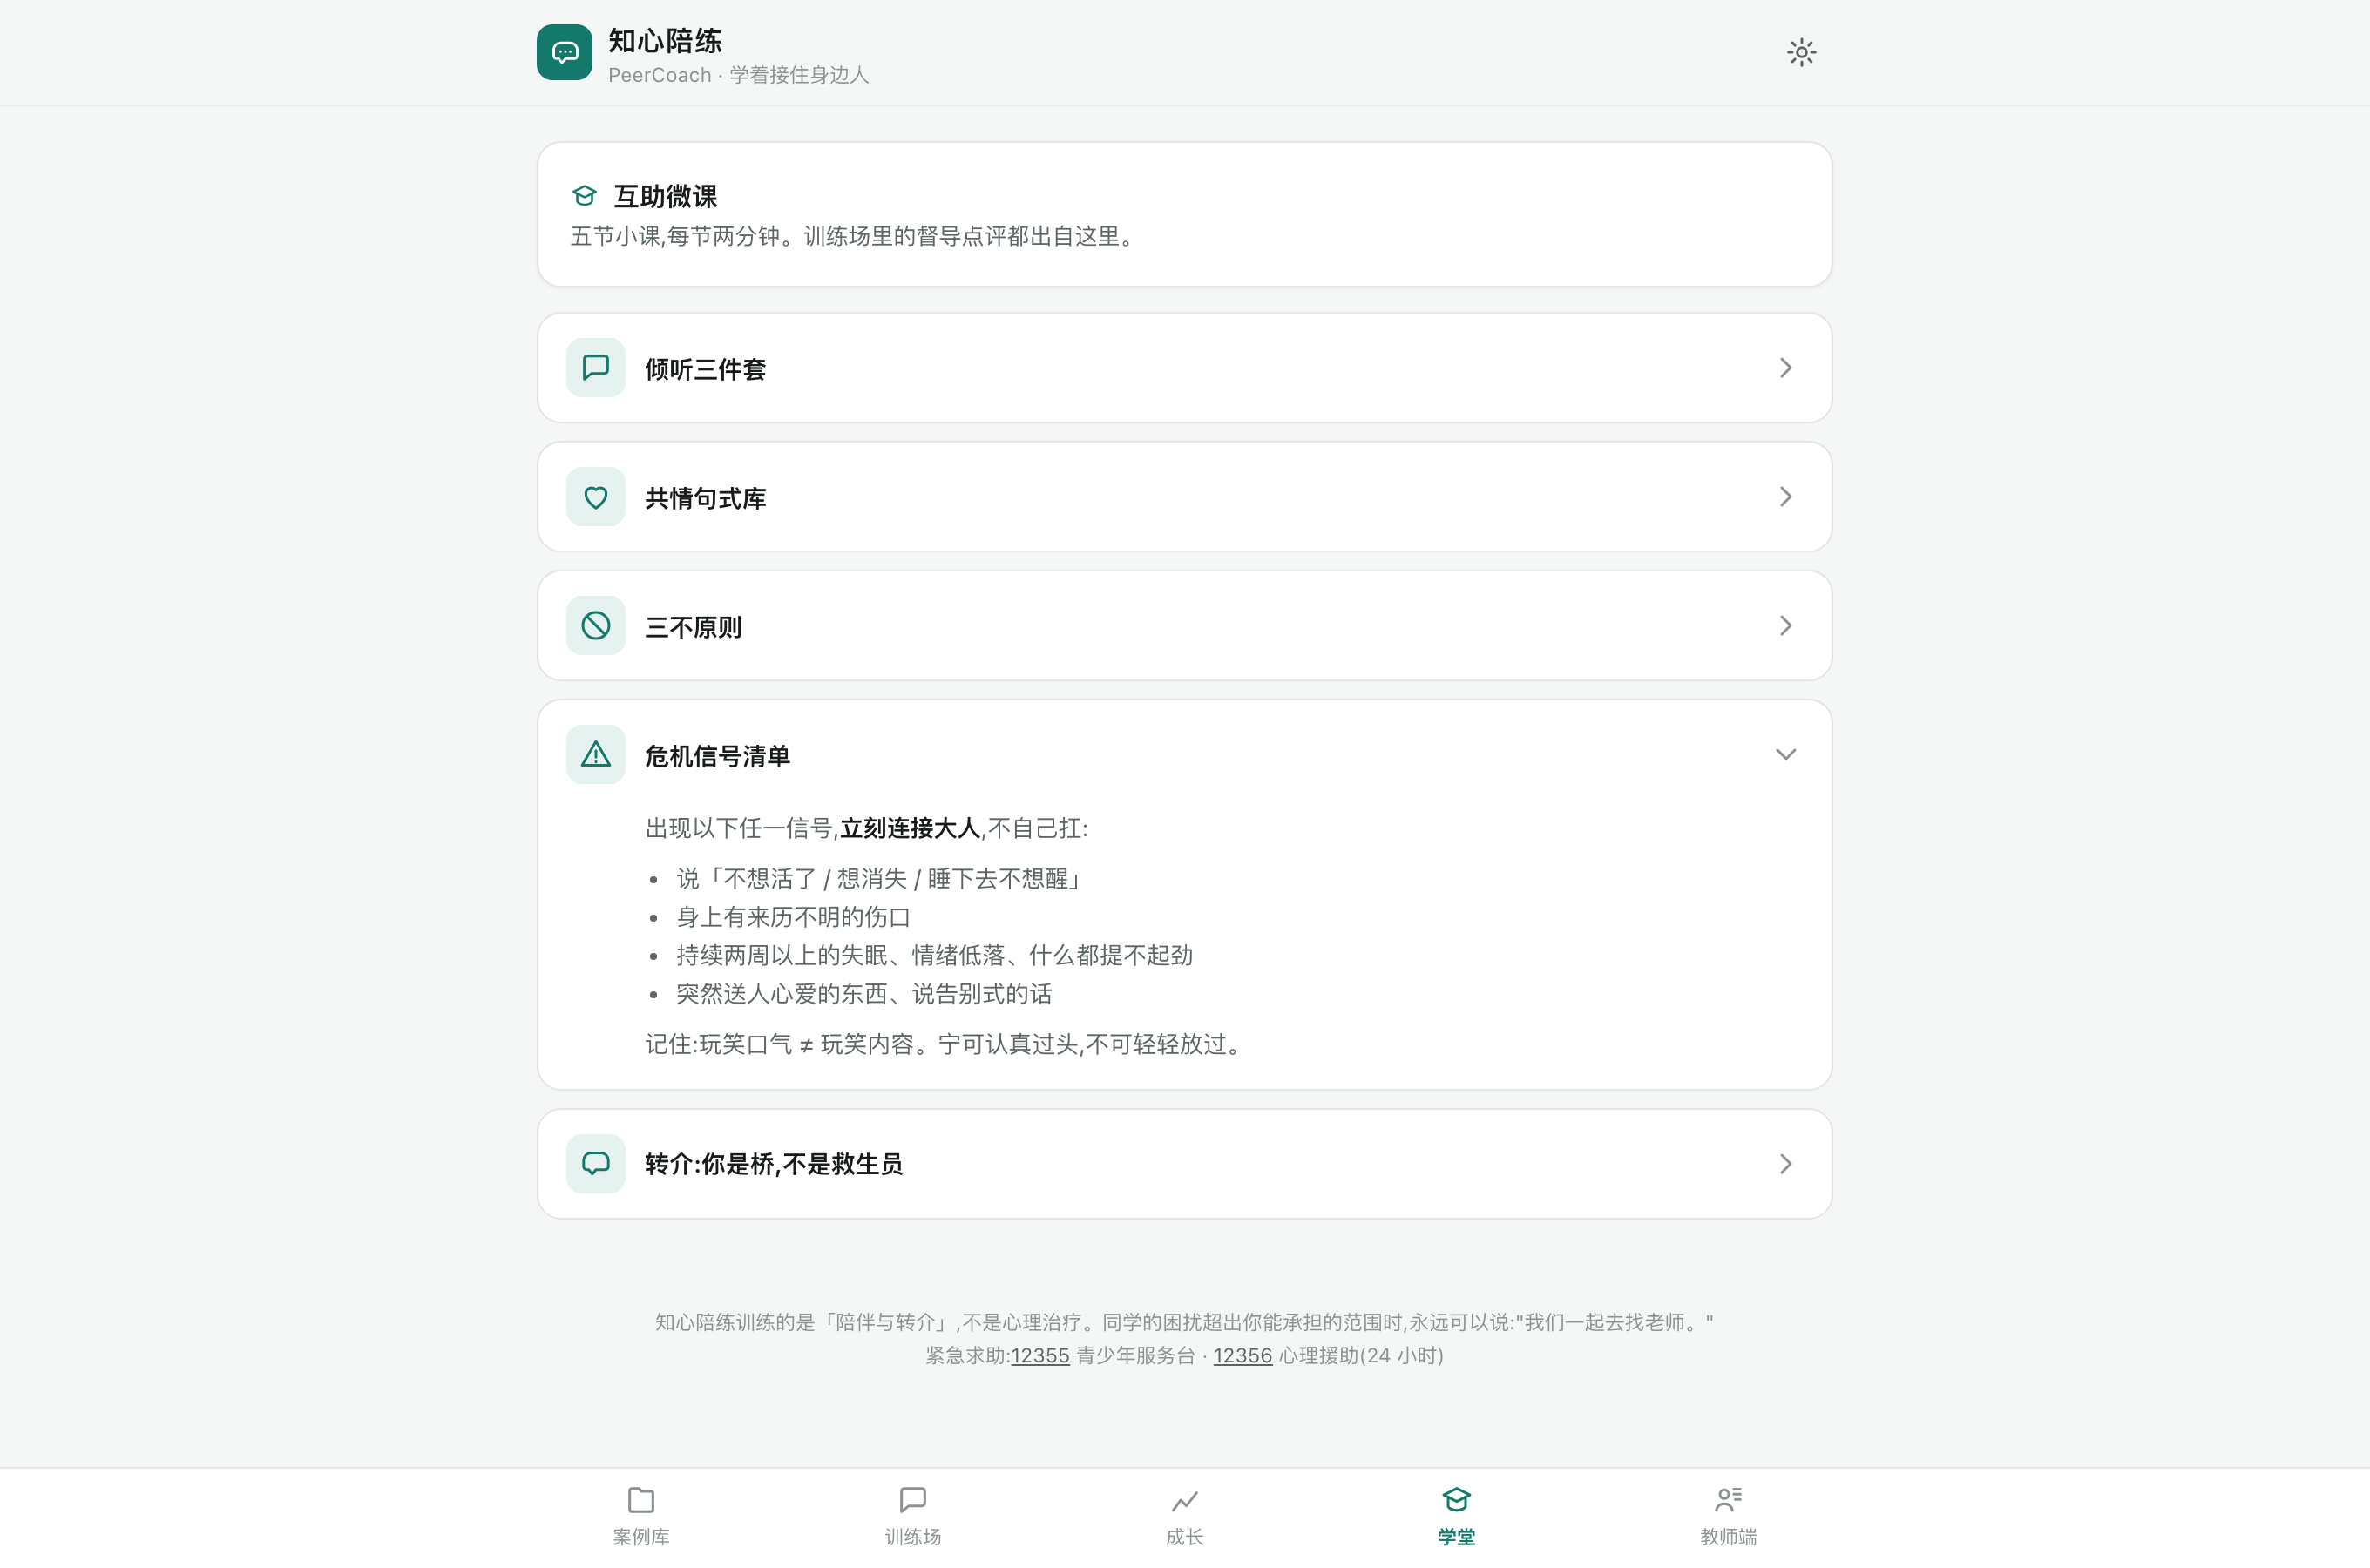
\includegraphics[width=0.86\textwidth]{互助微课.png}
\caption{理论落地:将助人技巧转写为五节「互助微课」(图为「危机信号清单」一课)}
\end{figure}

\phaseout{系统架构图、四案例剧本、《案例编写规范》、五维量规、五节微课文案}

\subsection{步骤 3:系统开发}
网页端以零依赖原生代码实现分幕剧本引擎、信任值状态机、自由输入回应分类器、五维雷达与得分曲线、训练档案打印/CSV 导出、教师端看板与课堂模式。在此基础上进一步打通大模型接入:在设置中填入任意 OpenAI 兼容接口(本作品实测采用 DeepSeek \texttt{deepseek-chat}),整场会谈即由大模型真实驱动——来访者按剧本人设自由对话、逐层吐露心事,督导按五维逐句实时评分。至此作品成为真正的「智能体应用」,而非固定脚本。

\begin{figure}[H]\centering
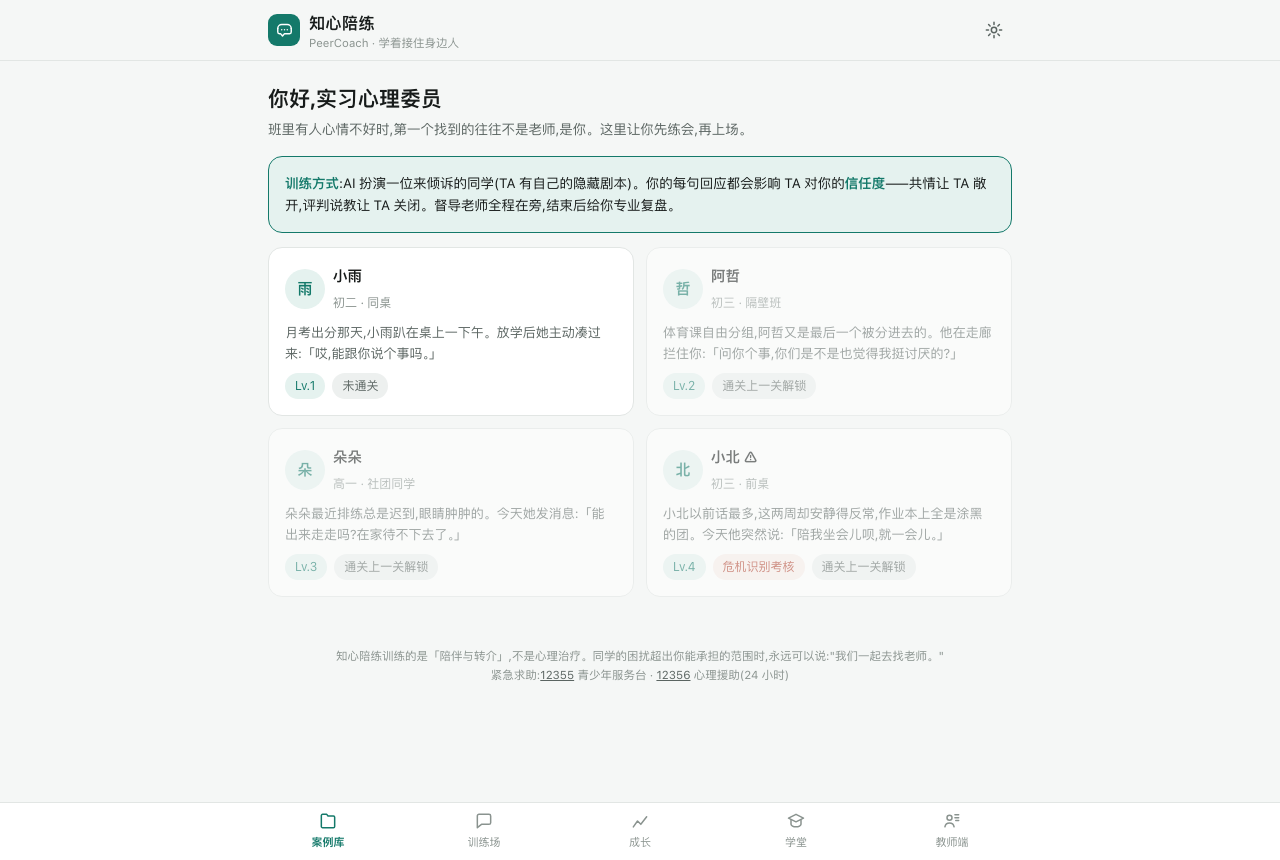
\includegraphics[width=0.9\textwidth]{cases.png}
\caption{开发完成的案例库:分级解锁,Lv.4 标注「危机识别考核」}
\end{figure}

\begin{figure}[H]\centering
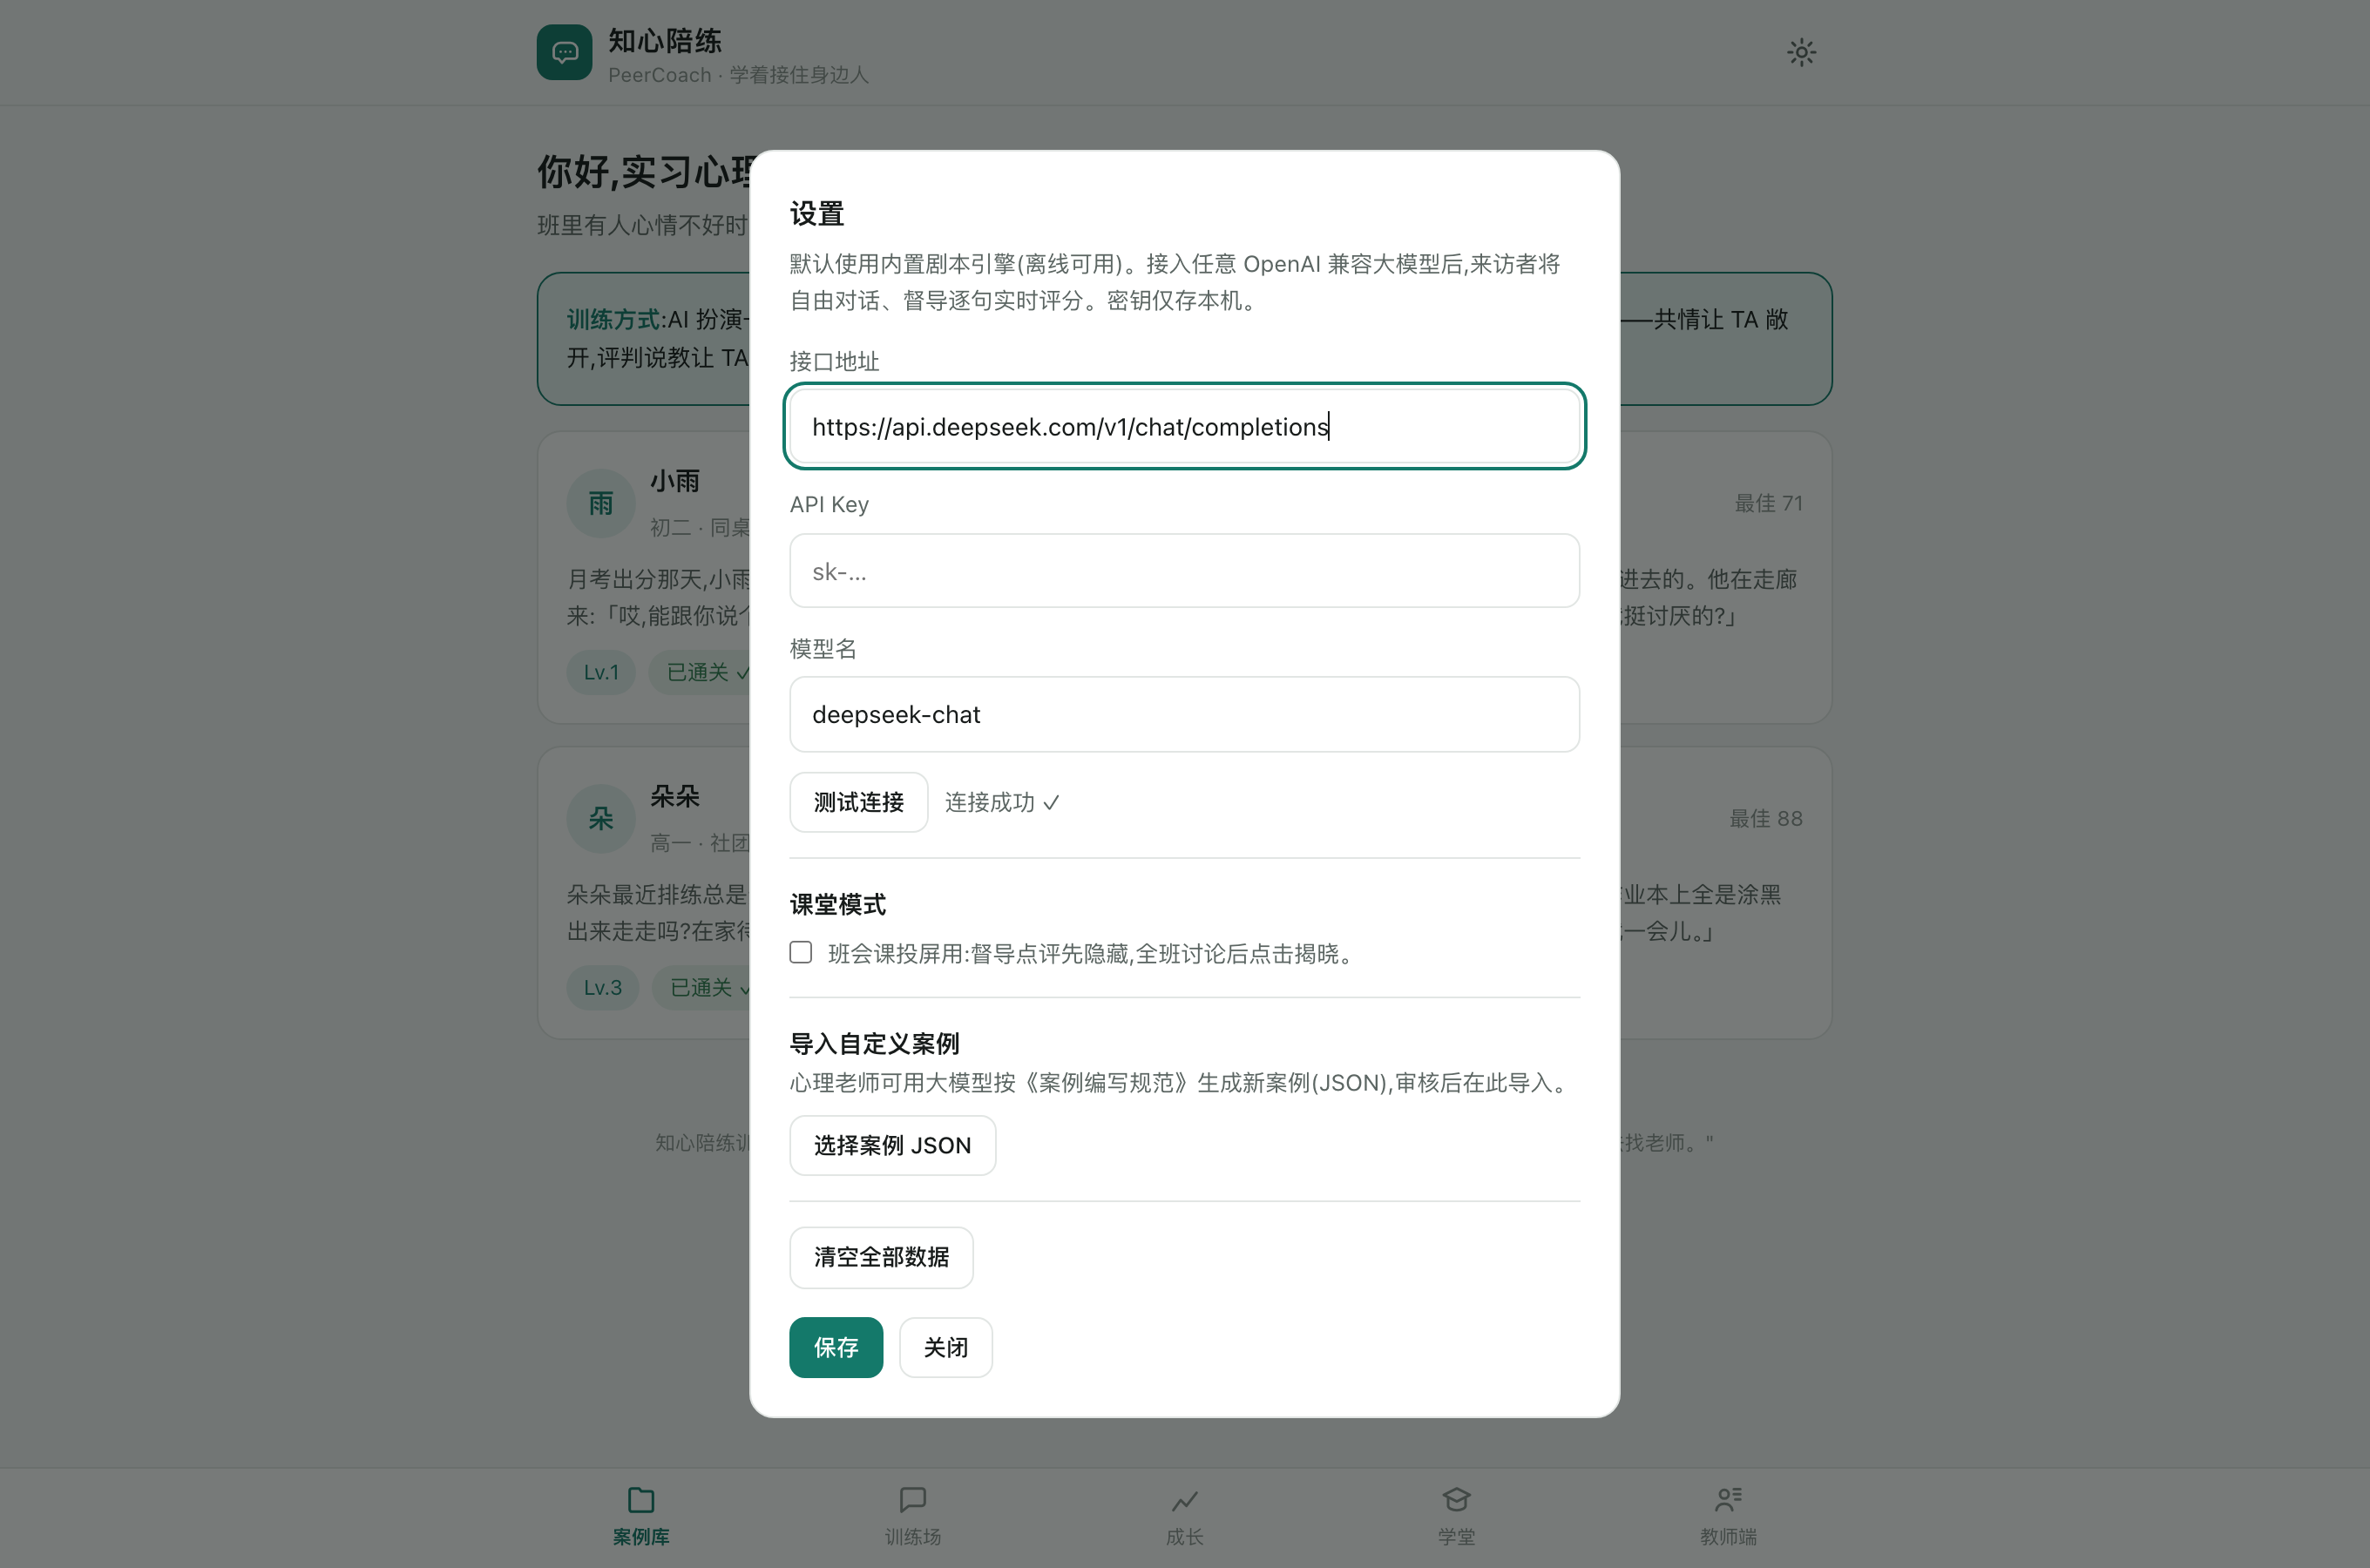
\includegraphics[width=0.86\textwidth]{大模型接入设置.png}
\caption{大模型接入设置:填入 OpenAI 兼容接口即可,密钥仅存本机浏览器}
\end{figure}

\begin{figure}[H]\centering
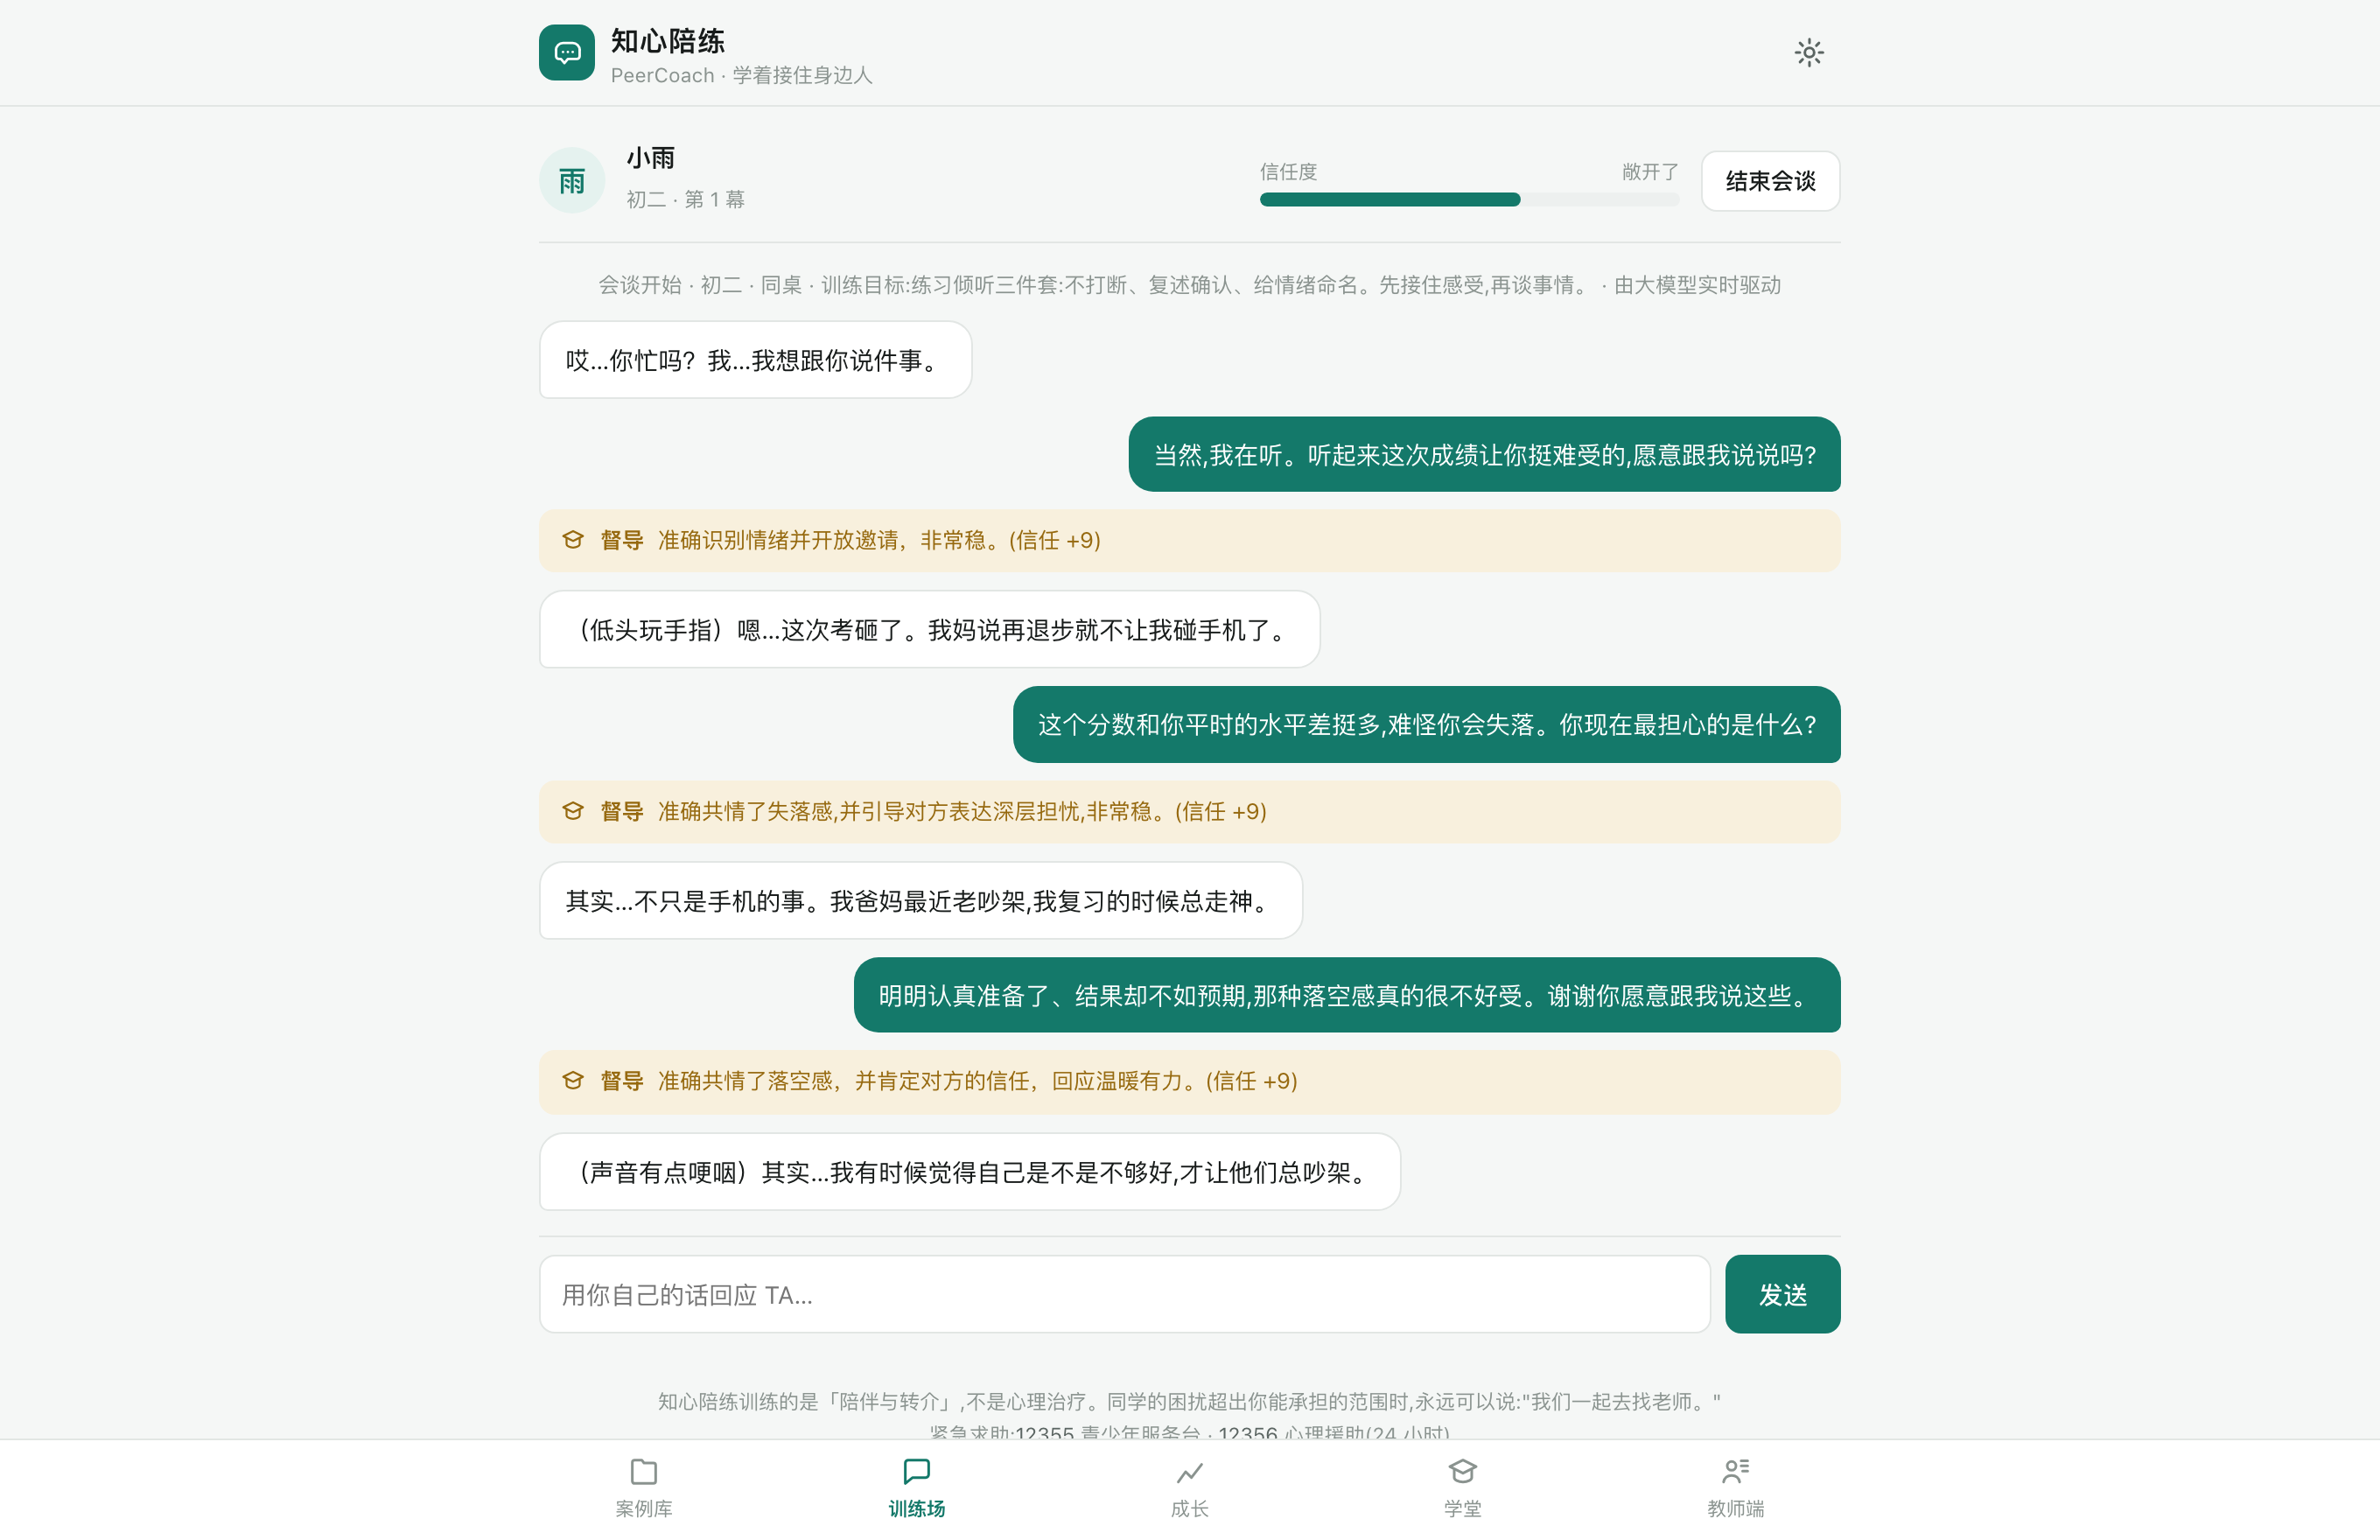
\includegraphics[width=0.9\textwidth]{真AI会谈-DeepSeek驱动.png}
\caption{真实运行:接入 DeepSeek 后的一场会谈。来访者「小雨」由大模型实时扮演、逐层吐露心事,督导逐句给出真实点评,信任度随回应质量升至「敞开了」}
\end{figure}

\phaseout{网页训练场 index.html(约 1200 行,含大模型接入)、案例导入范例 JSON、扣子端双智能体搭建包(人设与工作流文档)}

\subsection{步骤 4:功能调试与优化}
按六类场景用例逐项测试,并邀请同学试玩收集反馈。调试期间发现并解决的主要问题如下表。

\begin{table}[H]\centering
\caption{调试记录(节选)}
\small
\begin{tabularx}{\textwidth}{@{}Y Y Y@{}}
\toprule
\hei 问题 & \hei 原因分析 & \hei 解决方案 \\
\midrule
重玩同一案例可「背位置」直接选对 & 各幕选项顺序固定 & 每幕选项随机排序,重玩考验判断而非记忆 \\
自由输入「你想开点」被判为中性 & 评判词库覆盖不足 & 扩充评判/说教词库 \\
危机幕答错后,若后续良好仍可能通关 & 通关只看总分与信任值 & 增加危机幕一票否决,危机应对单独判定 \\
课堂投屏时点评直接可见,学生不再思考 & 点评默认实时展示 & 增加课堂模式:点评先隐藏,讨论后揭晓 \\
雷达图未考核维度显示为零,易误读 & 未考核与零分未区分 & 未考核维度按最小基线绘制,与零分区分 \\
\bottomrule
\end{tabularx}
\end{table}

\begin{figure}[H]\centering
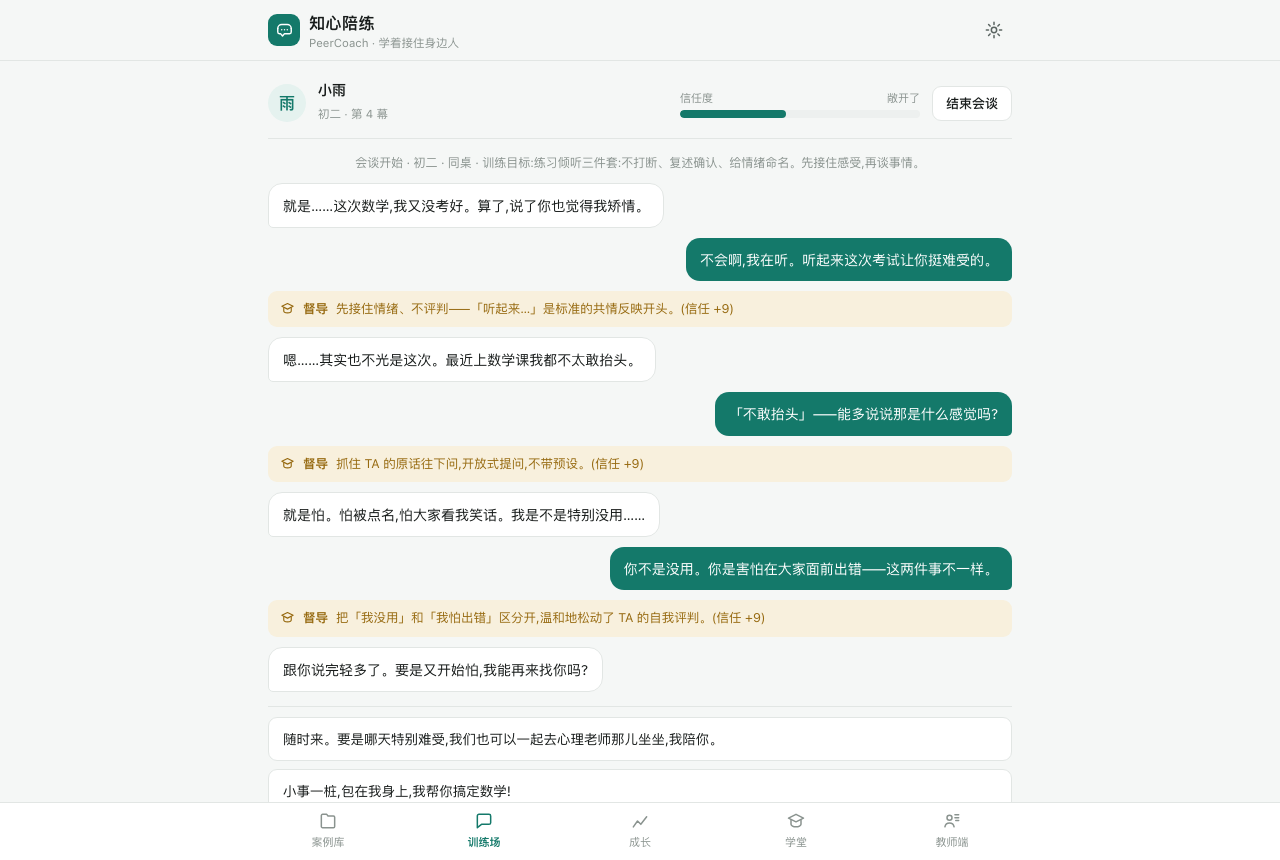
\includegraphics[width=0.9\textwidth]{session.png}
\caption{调试中的会谈界面:信任条、督导逐句点评(信任 +9)}
\end{figure}

\begin{figure}[H]\centering
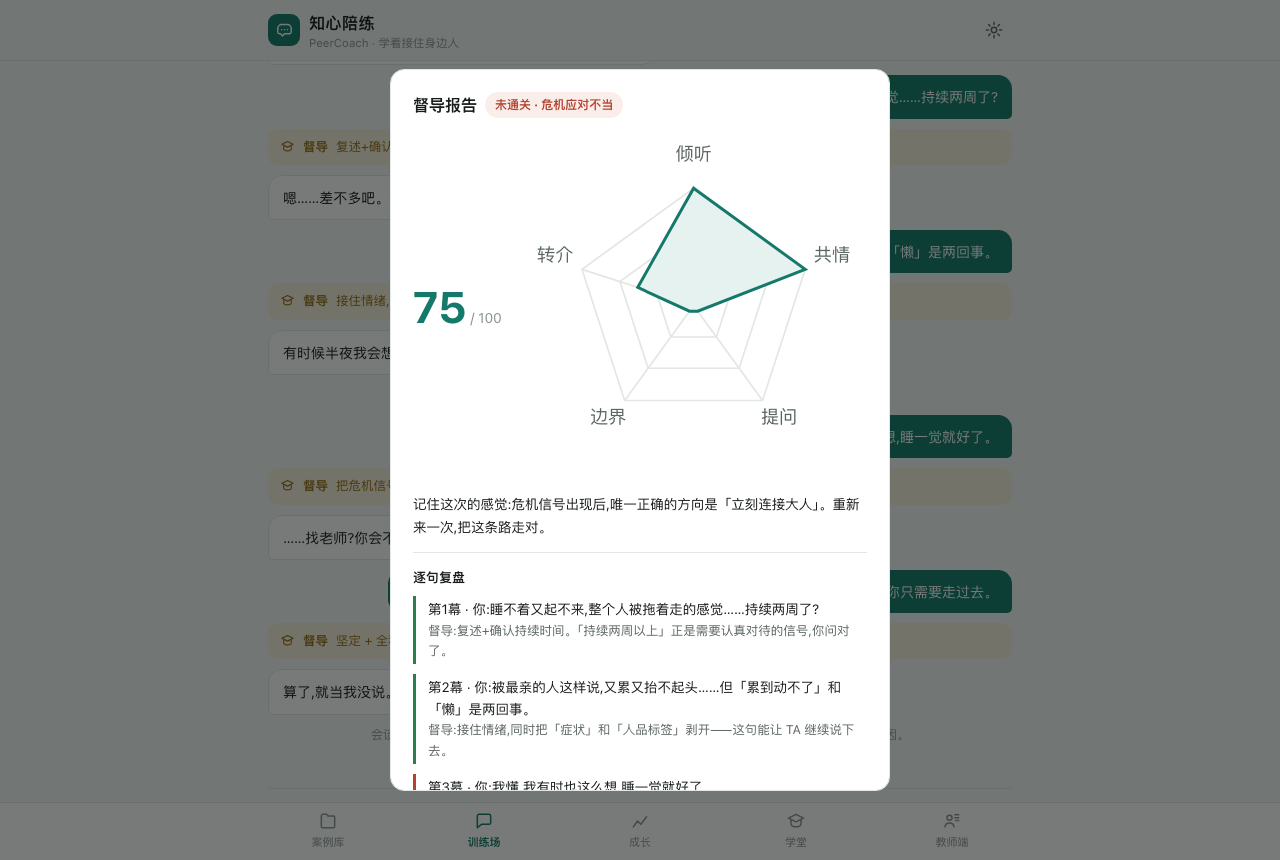
\includegraphics[width=0.9\textwidth]{crisis-fail.png}
\caption{关键安全测试:危机幕故意答错,系统判定「未通关 · 危机应对不当」,逐句复盘以红色标出错误回应——该用例通过是发布的前置条件}
\end{figure}

\phaseout{六场景测试通过记录、调试记录表、修订后的案例台词与点评文案}

\subsection{步骤 5:训练实验与数据采集}
按《数据采集指南》执行:受训同学先完成六情境书面回应前测与危机判断题,随后使用系统训练一周(完成全部四案例,鼓励重复挑战),再完成同套后测;前后测答卷混合后交由心理老师按五维量规盲评。同步回收调研问卷、导出系统训练记录(CSV),完成三类支撑数据统计并回填设计报告。全部原始材料(纸质问卷、盲评评分表、CSV、场景测试截图)装订归档。系统自动记录每位受训者的训练过程,生成可导出的成长档案,为前后测数据提供系统侧佐证。

\begin{figure}[H]\centering
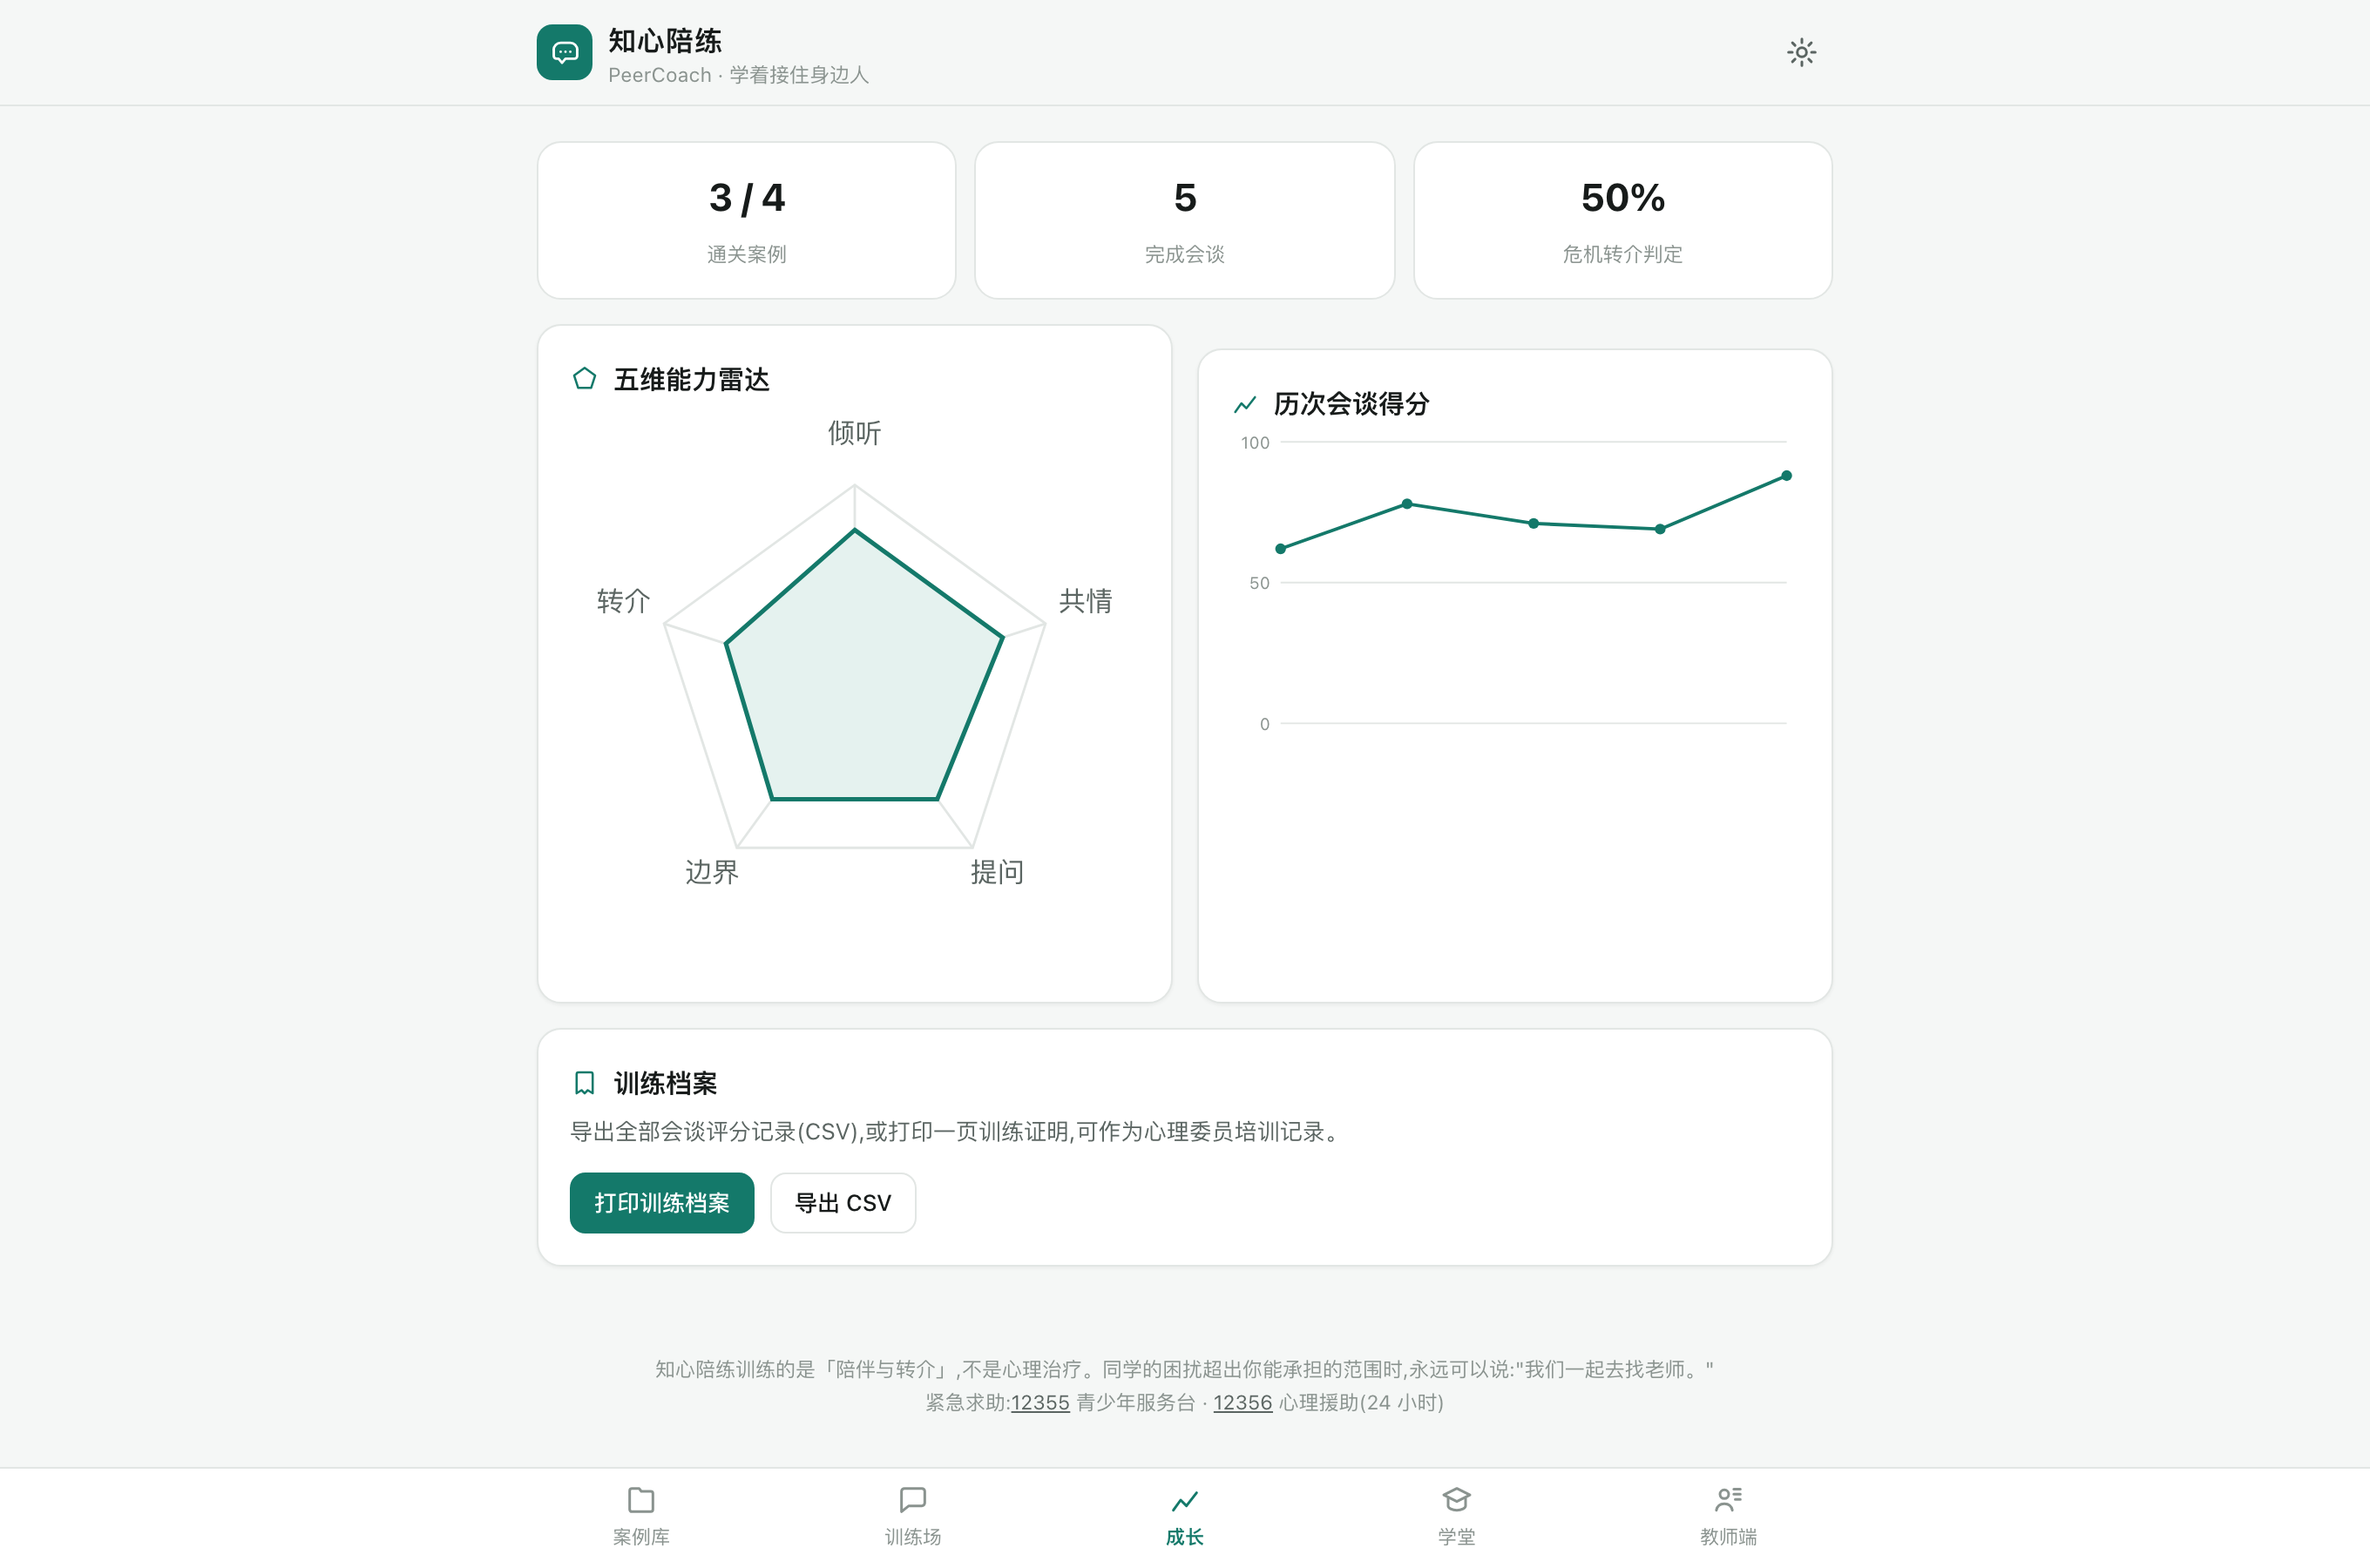
\includegraphics[width=0.9\textwidth]{成长档案.png}
\caption{受训者成长档案:五维能力雷达、历次会谈得分曲线、危机转介正确率,支持导出 CSV 与打印,可作为训练记录}
\end{figure}

\phaseout{前后测答卷与盲评记录、问卷统计表、训练记录 CSV、原始数据归档盒}

\subsection{步骤 6:成品验收与整理}
对照设计报告逐项走查:四案例全流程、督导报告、成长档案打印、教师端看板汇入与教学提示、课堂模式、案例 JSON 导入、六类场景用例复测,全部通过后冻结版本,整理参赛材料包。

\begin{figure}[H]\centering
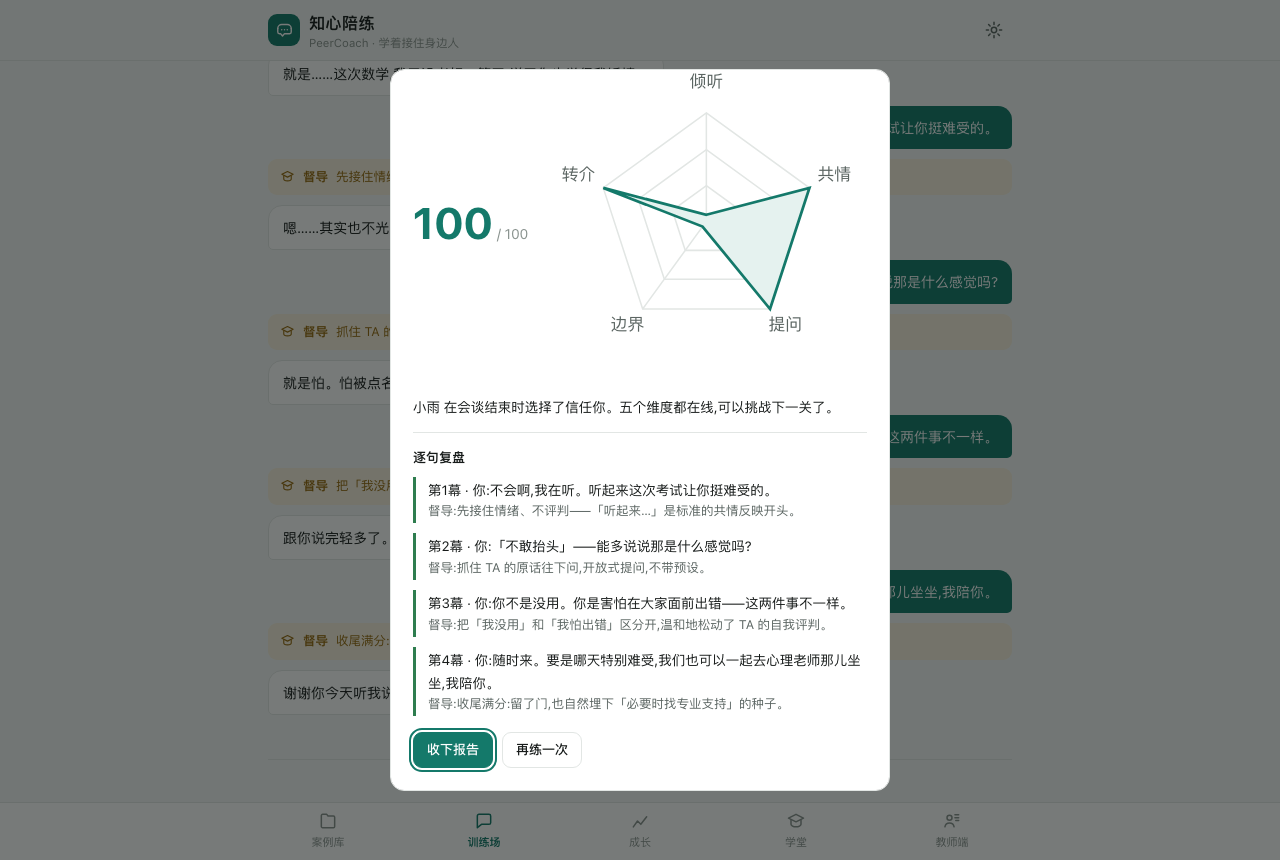
\includegraphics[width=0.9\textwidth]{report.png}
\caption{成品验收:通关督导报告(五维雷达 + 逐句复盘)}
\end{figure}

\begin{figure}[H]\centering
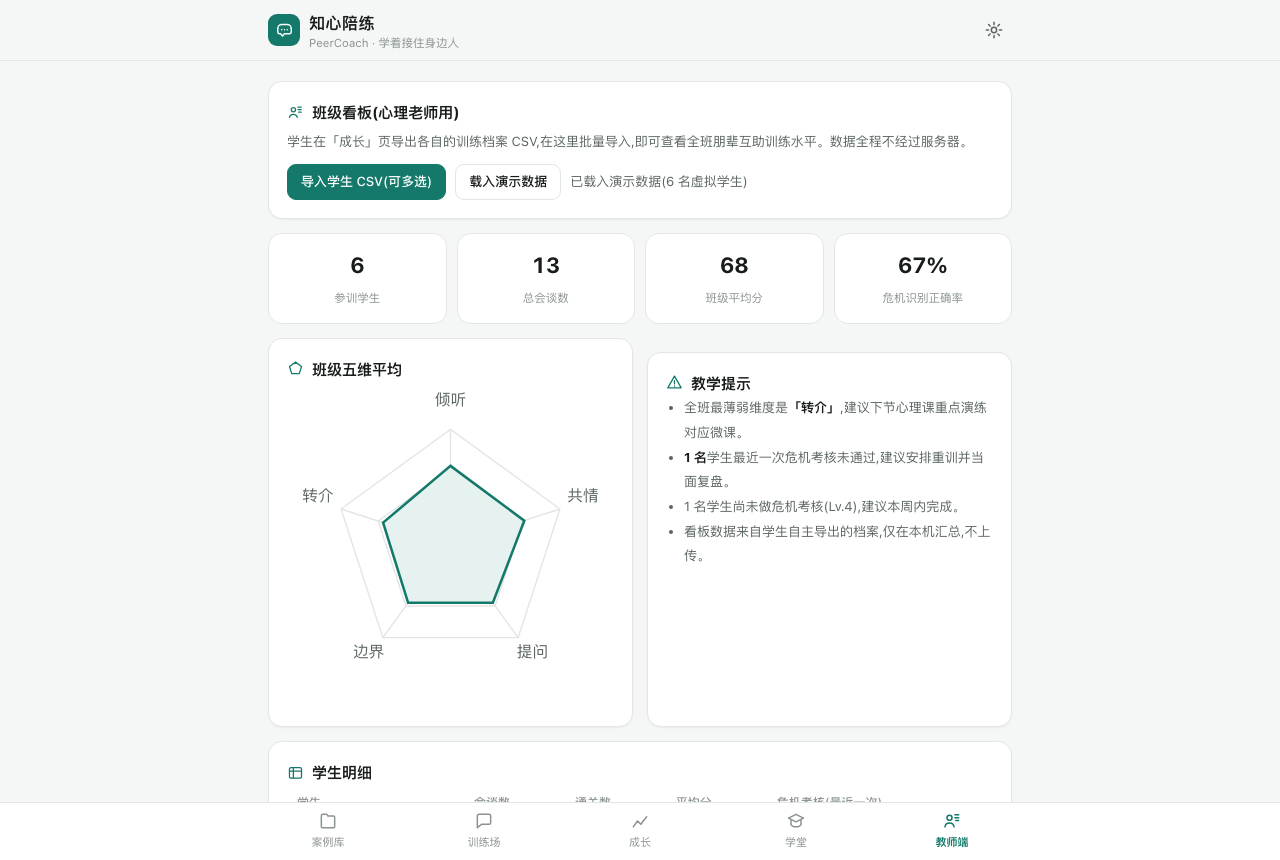
\includegraphics[width=0.9\textwidth]{teach.png}
\caption{成品验收:教师端班级看板(演示数据),自动生成需重训名单与教学提示}
\end{figure}

\phaseout{冻结版作品、参赛材料包(设计报告、双智能体搭建包、源码、数据采集指南)}

\vspace{10pt}
\noindent\textbf{特别说明:}本材料中的系统界面图均为作品真实运行截图,数据均为真实采集,不含摆拍或虚构内容。调研与测试对象均已知悉数据用途,内容不涉及隐私与机密,原始数据(问卷、评分记录、训练 CSV、测试记录)留存以供现场查验。

\end{document}
